
\pagestyle{fancy}%to add custom header & footer along with lines @ top & bottom
\fancyhf{} %clear default settings 
%the section name at the header will be of caps by default hence we need change 
\renewcommand{\chaptermark}[1]{%
         \markboth{#1}{}}
\renewcommand{\sectionmark}[1]{%
         \markright{\thesection\ #1}}
%put page mark at left of even page & right of odd page
\fancyhead[LE,RO]{\bfseries\thepage}
\fancyhead[LO]{\bfseries\rightmark}
\fancyhead[RE]{\bfseries\leftmark}
\pagenumbering{arabic}%add number in arabic style
\newpage%start contents from newpage
\renewcommand{\headrulewidth}{0.5pt}
\renewcommand{\footrulewidth}{0.5pt}

%%%%%%%%%%%%%%%%%%%%%%%%%
%start editing from here
%%%%%%%%%%%%%%%%%%%%%%%%%

%%Instructions for editing%%
%%There is sample code given below for adding figures,tables,code,etc
%%Use only those sections you need and delete the rest
%%Copy same sections at different locations in your report for usage at multiple locations
%%For any further queries contact us

%%%%%%%%%%%%%%%%%%%%%%%%%%%%%%%%%%%%%%%%%%%%%%%%%%%%%%%%%%%%%%%%%%%%%%
%creating sections as(1,2,3..) and subsections as(1.1,1.2...2.1,2.2..)
%%%%%%%%%%%%%%%%%%%%%%%%%%%%%%%%%%%%%%%%%%%%%%%%%%%%%%%%%%%%%%%%%%%%%% 
\section{Introduction}
	The Feature Finding Team (FFT) is an international consortium with the task to produce a comprehensive automated feature and event recognition system for SDO.
It provides several different modules to look at different features and events.
The flare detective is the module with the  task of detecting flares from AIA images
	\subsection{}
	\subsubsection{}

\section{Algorithm}

FFT modules works a bit differently then the way one would build such a module if all data was available
The flare detective is fed one image at a time
There is no options to retrieve that image at a later time
All relevant information about past images is stored in an internal status of the module
One instance of the flare detective works with images from one AIA channel (independently from other instances of the module that may be running on otehr channels)

The large AIA images are segmented in a small number of macropixels
Lightcurves are computed for each macropixels
Flares start times are determined when the derivative of the lightcurve reaches a certain threshold  
Flares end times are determined when the flux is lower then a certain fraction of the peak flux	

%%%%%%%%%%%%%%%%%%%%%
\begin{figure}%to start a figure environment
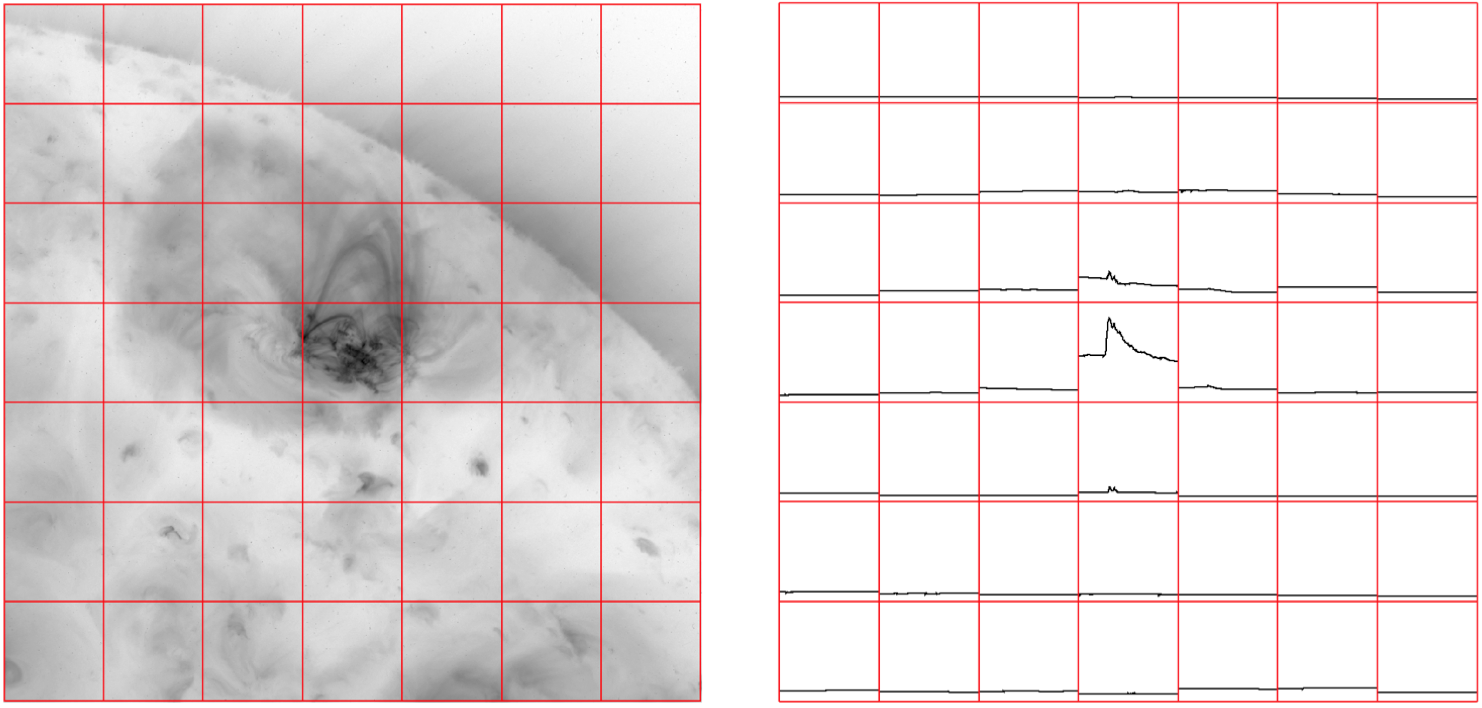
\includegraphics[scale=.27]{images/flare_bin.png}
\captionof{figure}{name of fig}
\end{figure}

%%%%%%%%%%%%%%%%%%%%%

%\subsection{IPTV}
%	Internet Protocol television (IPTV) is a system through which Internet television services are delivered using the architecture and networking methods of the Internet Protocol Suite over a packet-switched network infrastructure, e.g. the Internet and broadband Internet access networks, instead of being delivered through traditional radio frequency broadcast, satellite signal, and cable television.\cite{IPTV}\\

%%%%%%%%%%%%%%%%%%%%%%%%%%%%%%%%%%%%%%%%%%%%%%%%%%%%%%%%%%%%%%%%%%%%%%
%For creating bulleted contents(itemize), numbered contents(enumarate),
%and contents with your own lables(description)
%%%%%%%%%%%%%%%%%%%%%%%%%%%%%%%%%%%%%%%%%%%%%%%%%%%%%%%%%%%%%%%%%%%%%%
\section{Itemize environment}







\begin{itemize}%itemize environment
\item .....
\item ....
\end{itemize}

\section{Enumerate}
\begin{enumerate}%numerate the items
\item.....
\item.....
\end{enumerate}

%\begin{description}%highlight the word within [], useful for writing glosarry
%\item[]....
%\item[]....
%\end{description}

%%%%%%%%%%%%%%%%%%%%%
%For inserting figures
%%%%%%%%%%%%%%%%%%%%%
\begin{figure}%to start a figure environment
%\includegraphics[scale factor]{image location}
%\captionof{figure}{name of fig}
\end{figure}

%%%%%%%%%%%%%%%%%%%%%
%For inserting tables
%%%%%%%%%%%%%%%%%%%%%
\section{tabular}
\begin{tabular}{|c|c|c|}\hline%here, table with 3 columns is given..for 4 coulmns, change to |c|c|c|c|..etc 
x & y & z\\ \hline %'&'seperate the different column entry.\hline adds horizontal line
a & b &c \\ \hline % x,y,z,a,b,c are elements of table
\end{tabular}

%%%%%%%%%%%%%%%%%%%%%%%%%%%%%%%
%For including your c code files
%%%%%%%%%%%%%%%%%%%%%%%%%%%%%%%
%\lstset{language=[ANSI]C}%specify the type of source code
%\lstinputlisting{path of code file}
